% !TeX encoding = UTF-8
\documentclass[a4paper,12pt]{article}
\usepackage{ctex,geometry,graphicx,tikz,setspace,paralist,fancyhdr,caption,ulem}
\geometry{
	left=1.5cm,
	right=1.5cm,
	top=1.3cm,
	bottom=2cm,}
\newcommand{\rec}{
	\begin{tikzpicture}[remember picture,overlay]
		% 绘制边框
		\draw[line width=1.2pt] ([xshift=0.5cm,yshift=0.5cm] current page.south west) rectangle ([xshift=-0.5cm,yshift=-0.8cm] current page.north east);
	\end{tikzpicture}
	
}
\renewcommand{\maketitle}{
	\begin{titlepage}
		\begin{center}
			
\includegraphics[width=0.4\textwidth]{1-1.png} % 插入你的公司/机构logo
			\vspace{2cm}
			
			\zihao{-0} \textbf{电子电路实习 \\ 课程期末报告} \\
			\vspace{2cm}
			\zihao{1} \textbf{——基于555芯片的 \\ \qquad 亮度调节器} \\
			\vspace{2cm}
			
			\zihao{2} 专业:\uline{通信工程} \\
			\zihao{2} 学号:\uline{22309080} \\
			\zihao{2} 姓名:\uline{梁倍铭} \\
			\zihao{2} 时间:\uline{2023.11.6} \\
			
			\vfill
		\end{center}
	\end{titlepage}
}
\pagestyle{fancy}
\fancyhf{}
\fancyhead[C]{\rec}  % 在页眉中绘制图形
\fancyhead[L]{电子电路实习报告}
\fancyhead[R]{基于555芯片的亮度调节器}
\fancyfoot[C]{\thepage}
\begin{document}
	\maketitle
	\large
	\onehalfspacing
	\section*{一、实验原理}
	\begin{enumerate}
		\item 555定时器原理简介 \par 
		\qquad555定时器是一种多用途的,集数字、模拟于一体的中规模集成电路,其应用极为广泛。它不仅用于信号的产生和变换,还常用于控制和检测电路中。由于使用灵活、方便,故而在波形的产生与交换、测量与控制、家用电器、电子玩具等许多领域中都得到了广泛应用。\par 
		\qquad555定时器分为双极型和CMOS两种类型,它们的结构及其工作原理基本相同岁,没有本质的区别。一般来说,双极型定时器的驱动能力较强,电源电压范围为5~16V,最大的负载电流可以达到200 mA。而CMOS定时器的电源电压范围为3~18V,最大负载电流在4 mA一下,它具有功耗低、输入阻抗高等优点。\par 
		\qquad 引脚图如下:\par 
		\begin{figure}[h]
			\centering
			\includegraphics[width=0.5\textwidth]{2.jpg}
			\caption*{图1 555引脚图}
		\end{figure}
		\qquad 引脚功能如下:
		\begin{enumerate}
			\item 1脚:接地。
			\item 2脚:输入端Trigger,该脚会判断其电压是否小于1/3 Vcc。
			\item 3脚:输出端Output。
			\item 4脚:清零端Reset。正常工作时应接高电平。
			\item 5脚:控制电压端。一般不使用,应通过一只0.01μF(103)瓷片电容接地,以防引入高频干扰。
			\item 6脚:输入端Threshold,该脚会判断其电压是否大于2/3 Vcc。
			\item 7脚:放电端Discharge。
			\item 8脚:外接电源Vcc,范围为4.5V~16V,一般用5V。
		\end{enumerate}
		\item PCB实验室制版流程:\par 
		\begin{enumerate}
			\item 原理图设计:设计完成的电路图经过仿真验证后用AD生成电路图,准备印制
			\item 热转印:将PCB图打印到黄油纸上,再将黄油纸上电路热转印到覆铜板上
			\item 腐蚀:将覆铜板没有电路的铜腐蚀掉
			\item 打孔:对于直插元件的焊盘,需要用打孔机打孔
			\item 除碳:用碳粉清洁剂清洁线路上覆盖的碳粉
			\item 焊接:按照设计的原理图进行焊接
		\end{enumerate}	
		\item 电路设计及原理简介 \par
		\begin{figure}[h]
			\centering
			\begin{minipage}{0.5\textwidth}
				\includegraphics[width=\textwidth]{2.png}
				\caption*{图2 电路原理图}
			\end{minipage}
			\qquad
			\begin{minipage}{0.5\textwidth}
				
\includegraphics[width=\textwidth]{3.png}
				\caption*{图3 电路PCB图}
			\end{minipage}
		\end{figure}
		\qquad 电路原理图如图2所示, PCB图如图3所示,光敏电阻和滑动变阻器作为电路的主要调节器件,光敏电阻的阻值会随着环境光线的变化而改变,而滑动变阻器与光敏电阻并联,可以调节电路对环境的敏感度。两者接入电源后连到放电端,同时通过二极管连入555芯片的输入段。\par 
		\qquad 555芯片将电压与Vcc比较,在输出端进行输出,控制发光二级管亮度。光敏电阻和滑动变阻器并联阻值的改变,影响着充电速度,进而影响输出波形的占空比\par 
		\item 元器件表\par 
		\qquad NE555芯片,发光二极管,光敏电阻,1N4007,直插电阻560k、1k、10k,瓷片电容20pf
	\end{enumerate}
	\section*{二、实验过程}
	\begin{enumerate}
		\item 确定电路功能,确定元件种类和参数\par 
		\qquad 参照了网上关于555定时器的介绍和实验室现有器件,从手机的自动亮度调节功能和路灯的自动开灯现象受到启发,最终确定题目为基于555芯片的亮度调节器。根据所需实现的功能,开始在protues中搭建电路仿真,并根据以下公式计算出电路中各个电阻的阻值:
		$$\mbox{占空比:}D=\frac{t_{\mbox{充}}}{T}$$
		$$t_{\mbox{充}}=0.693\frac{R_{\mbox{光敏电阻}} \times R_{\mbox{滑动变阻器}}}{R_{\mbox{光敏电阻}}+R_{\mbox{滑动变阻器}}}C$$
		\hspace{0.2cm}
		$$t_{\mbox{放}}=0.693R_2C_1$$
		$$T=t_{\mbox{充}}+t_{\mbox{放}}$$
		\item 仿真模拟,观察电路波形输出和实验现象\par 
		\qquad 在protues中搭建电路,进行测试。但是在仿真的过程中遇到了许多问题,比如一开始仿真的时候,电路没有充电电流,输出波形的占空比极小,如图4和图5所示。经过排查后是某一电容计算出错,接得太小,调整电容阻值后,得到了正确的仿真结果。\par 
		\qquad 在仿真过程中,还遇到了一个问题,就是在protues中找不到光敏电阻的阻值大小范围,最后我们通过去实验室测量,用滑动变阻器代替仿真,来得到较为准确的仿真结果,最后的仿真图如图6和图7所示。
		\begin{figure}[h]
			\centering
			\begin{minipage}{0.4\textwidth}
				\centering
				
\includegraphics[width=\textwidth]{4.png}
				\caption*{图4 仿真某一支路无电流}
			\end{minipage}
			\qquad
			\begin{minipage}{0.4\textwidth}
				\centering
				
\includegraphics[width=\textwidth]{5.png}
				\caption*{图5 仿真波形占空比极小}
			\end{minipage}
			\end{figure}
			\begin{figure}[h]
				\centering
				\begin{minipage}{0.4\textwidth}
					\centering
					\includegraphics[width=\textwidth]{6.png}
					\caption*{图6 最终仿真示意图}
				\end{minipage}
				\qquad
				\begin{minipage}{0.4\textwidth}
					\centering
					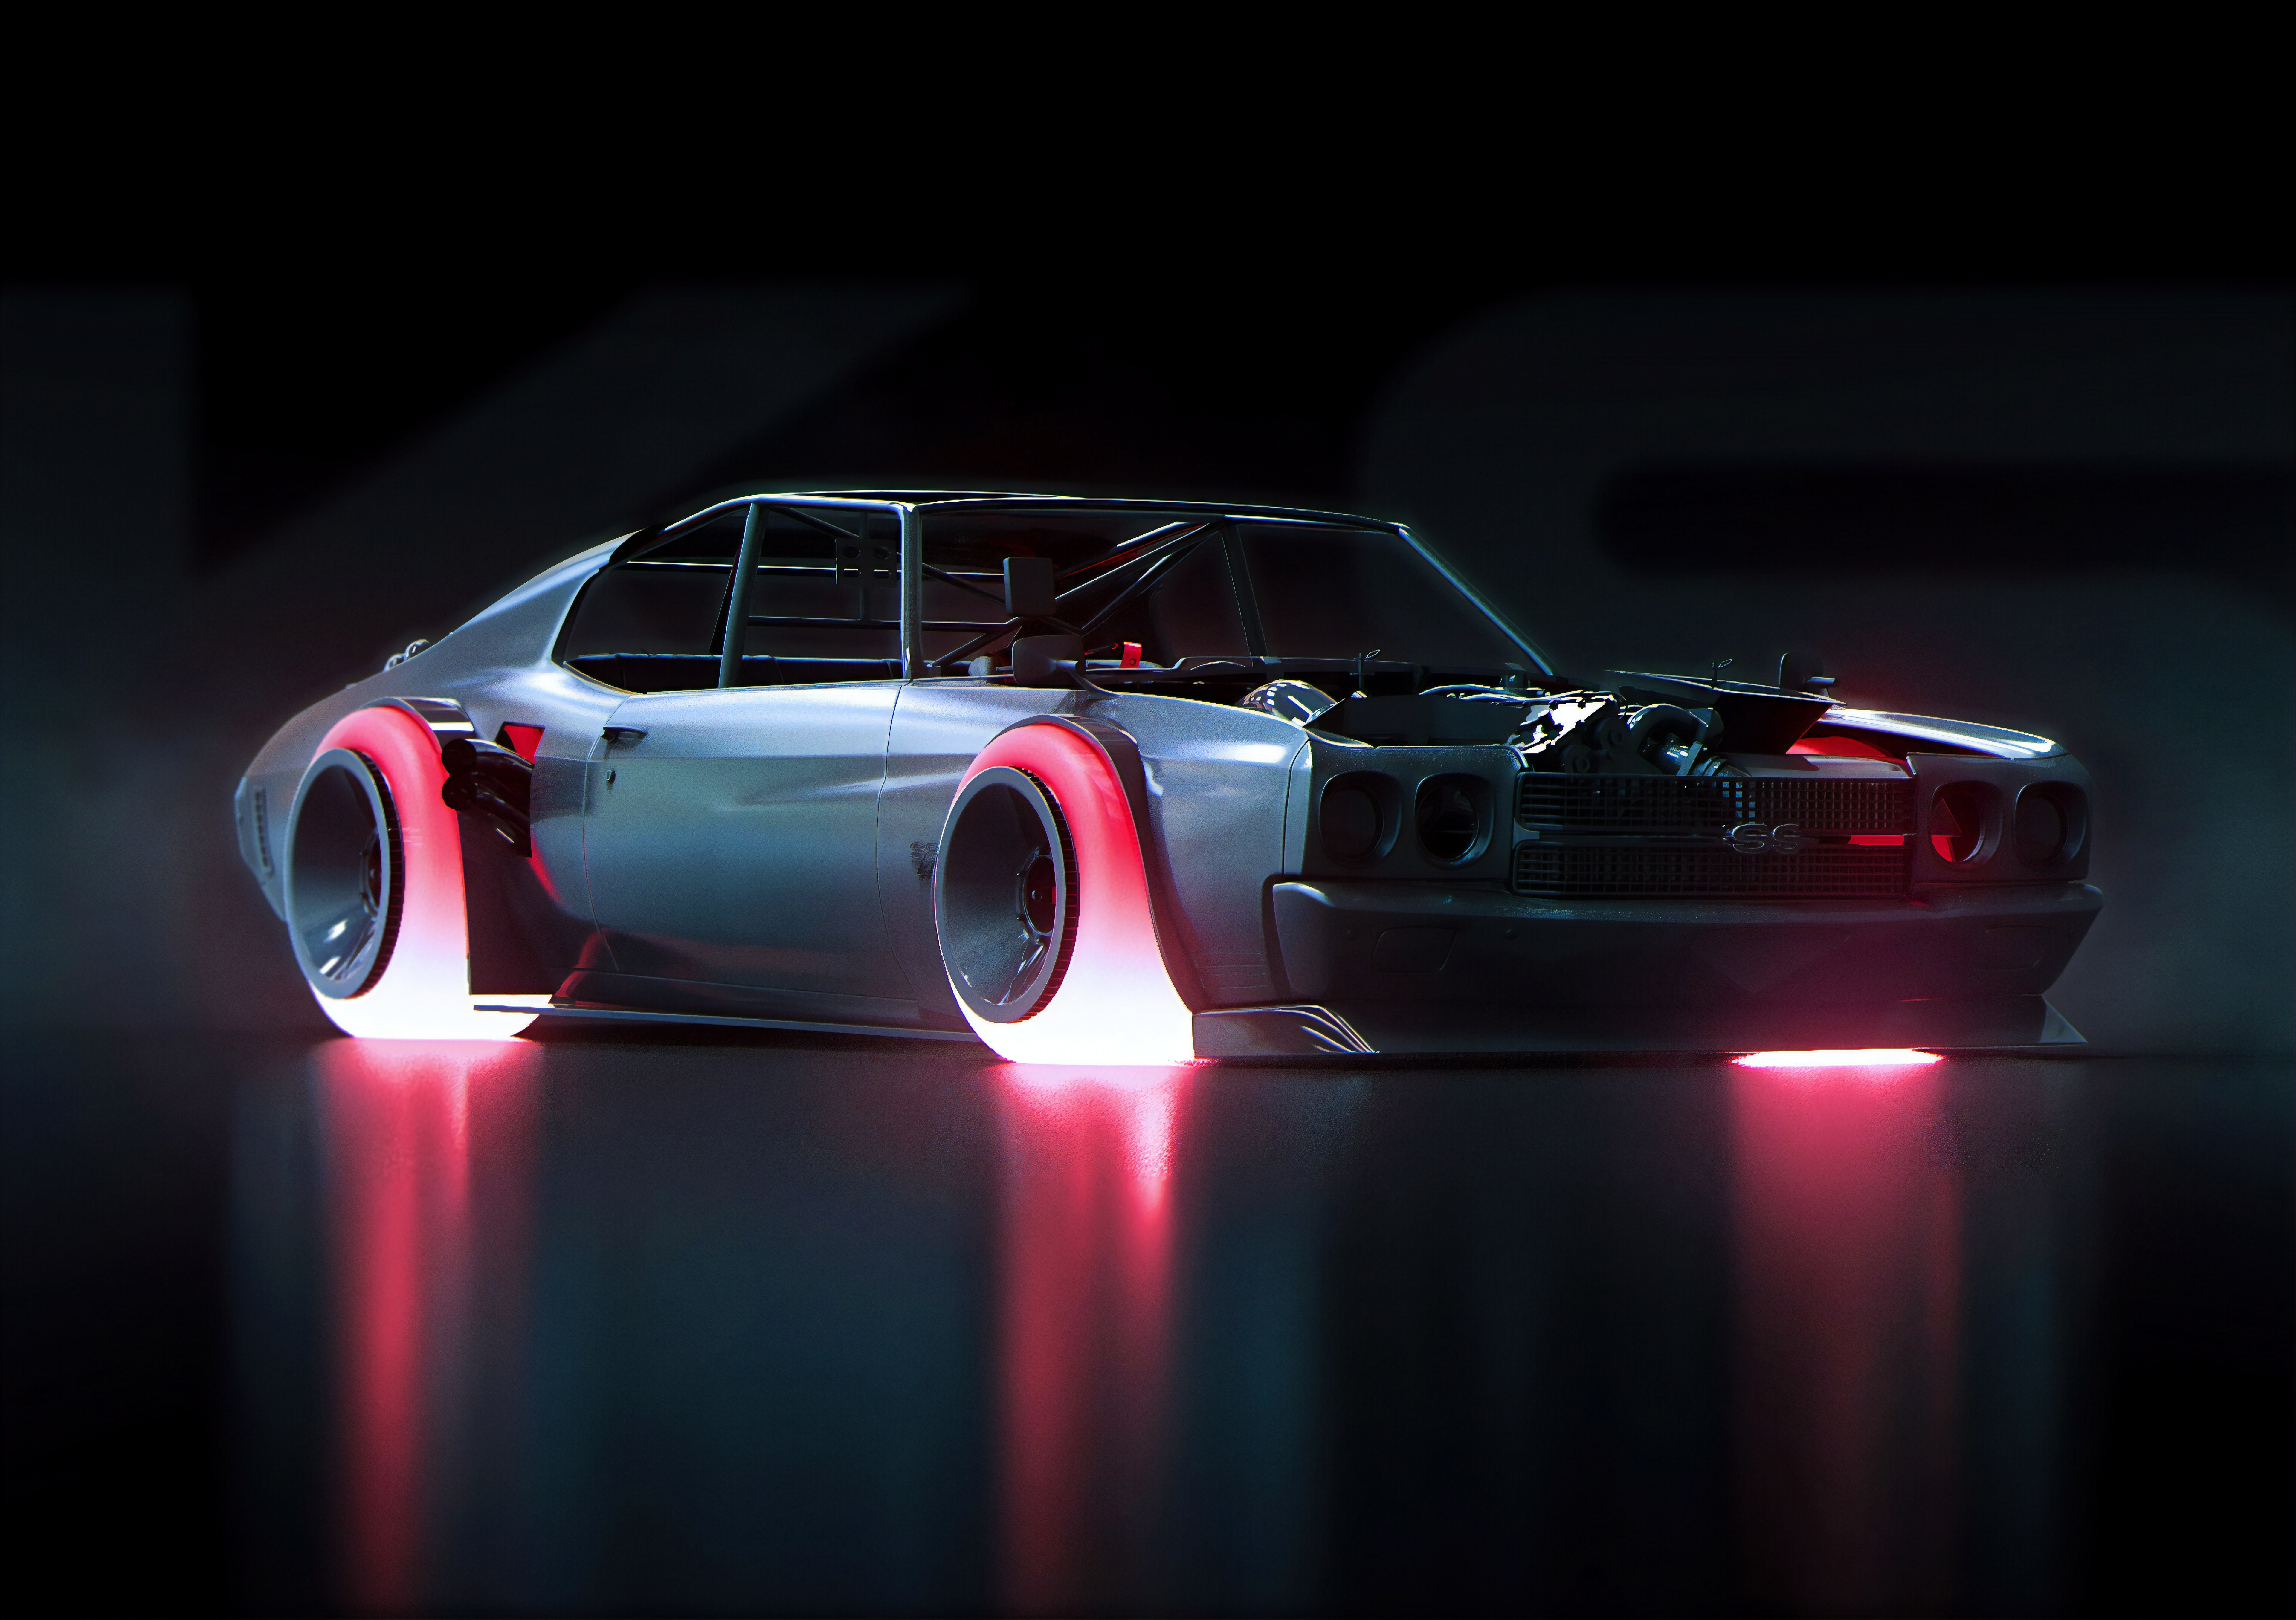
\includegraphics[width=\textwidth]{7.png}
					\caption*{图7 最终仿真输出波形}
				\end{minipage}
			\end{figure}
			\item 实验室制版并焊接元件 \par 
			\qquad 按照前面所述的制版流程,先从AD中导出PCB,然后将电路打印在黄油纸上(如图 8),在将黄油纸上的电路打印到覆铜板上(如图 9),最后在蚀刻机中将没有电路部分的铜腐蚀掉(如图 10),因为有直插元件,所以要在焊盘上打孔,根据不同的孔径大小选择不同直径的钻头(如图 11)。然后便是用碳粉清洁剂洗去碳粉,并根据原理图进行电路的焊接。 \par 
			\qquad 在制板的过程中,也出现了许多问题,比如第一次制板时发现导线太细,导线间的间距太小,后面在设计过程中加粗了布线宽度。\par 
			\qquad 最后焊接的成品如图12和图13所示。\par 
			\newpage
			\begin{figure}[h]
				\centering
				\begin{minipage}{0.35\textwidth}
					\centering
					
\includegraphics[width=\textwidth,height=0.3\textheight]{5.jpg}
					\caption*{图8 打印}
				\end{minipage}
				\qquad
				\begin{minipage}{0.35\textwidth}
					\centering
					\includegraphics[width=\textwidth,height=0.3\textheight]{6.jpg}
					\caption*{图9 热转印}
				\end{minipage}
				\\
				\begin{minipage}{0.35\textwidth}
					\centering
					
\includegraphics[width=\textwidth]{3.jpg}
					\caption*{图10 腐蚀}
				\end{minipage}
				\qquad
				\begin{minipage}{0.35\textwidth}
					\centering
					
\includegraphics[width=\textwidth]{4.jpg}
					\caption*{图11 打孔}
				\end{minipage}
				\\
				\begin{minipage}{0.35\textwidth}
					\centering
					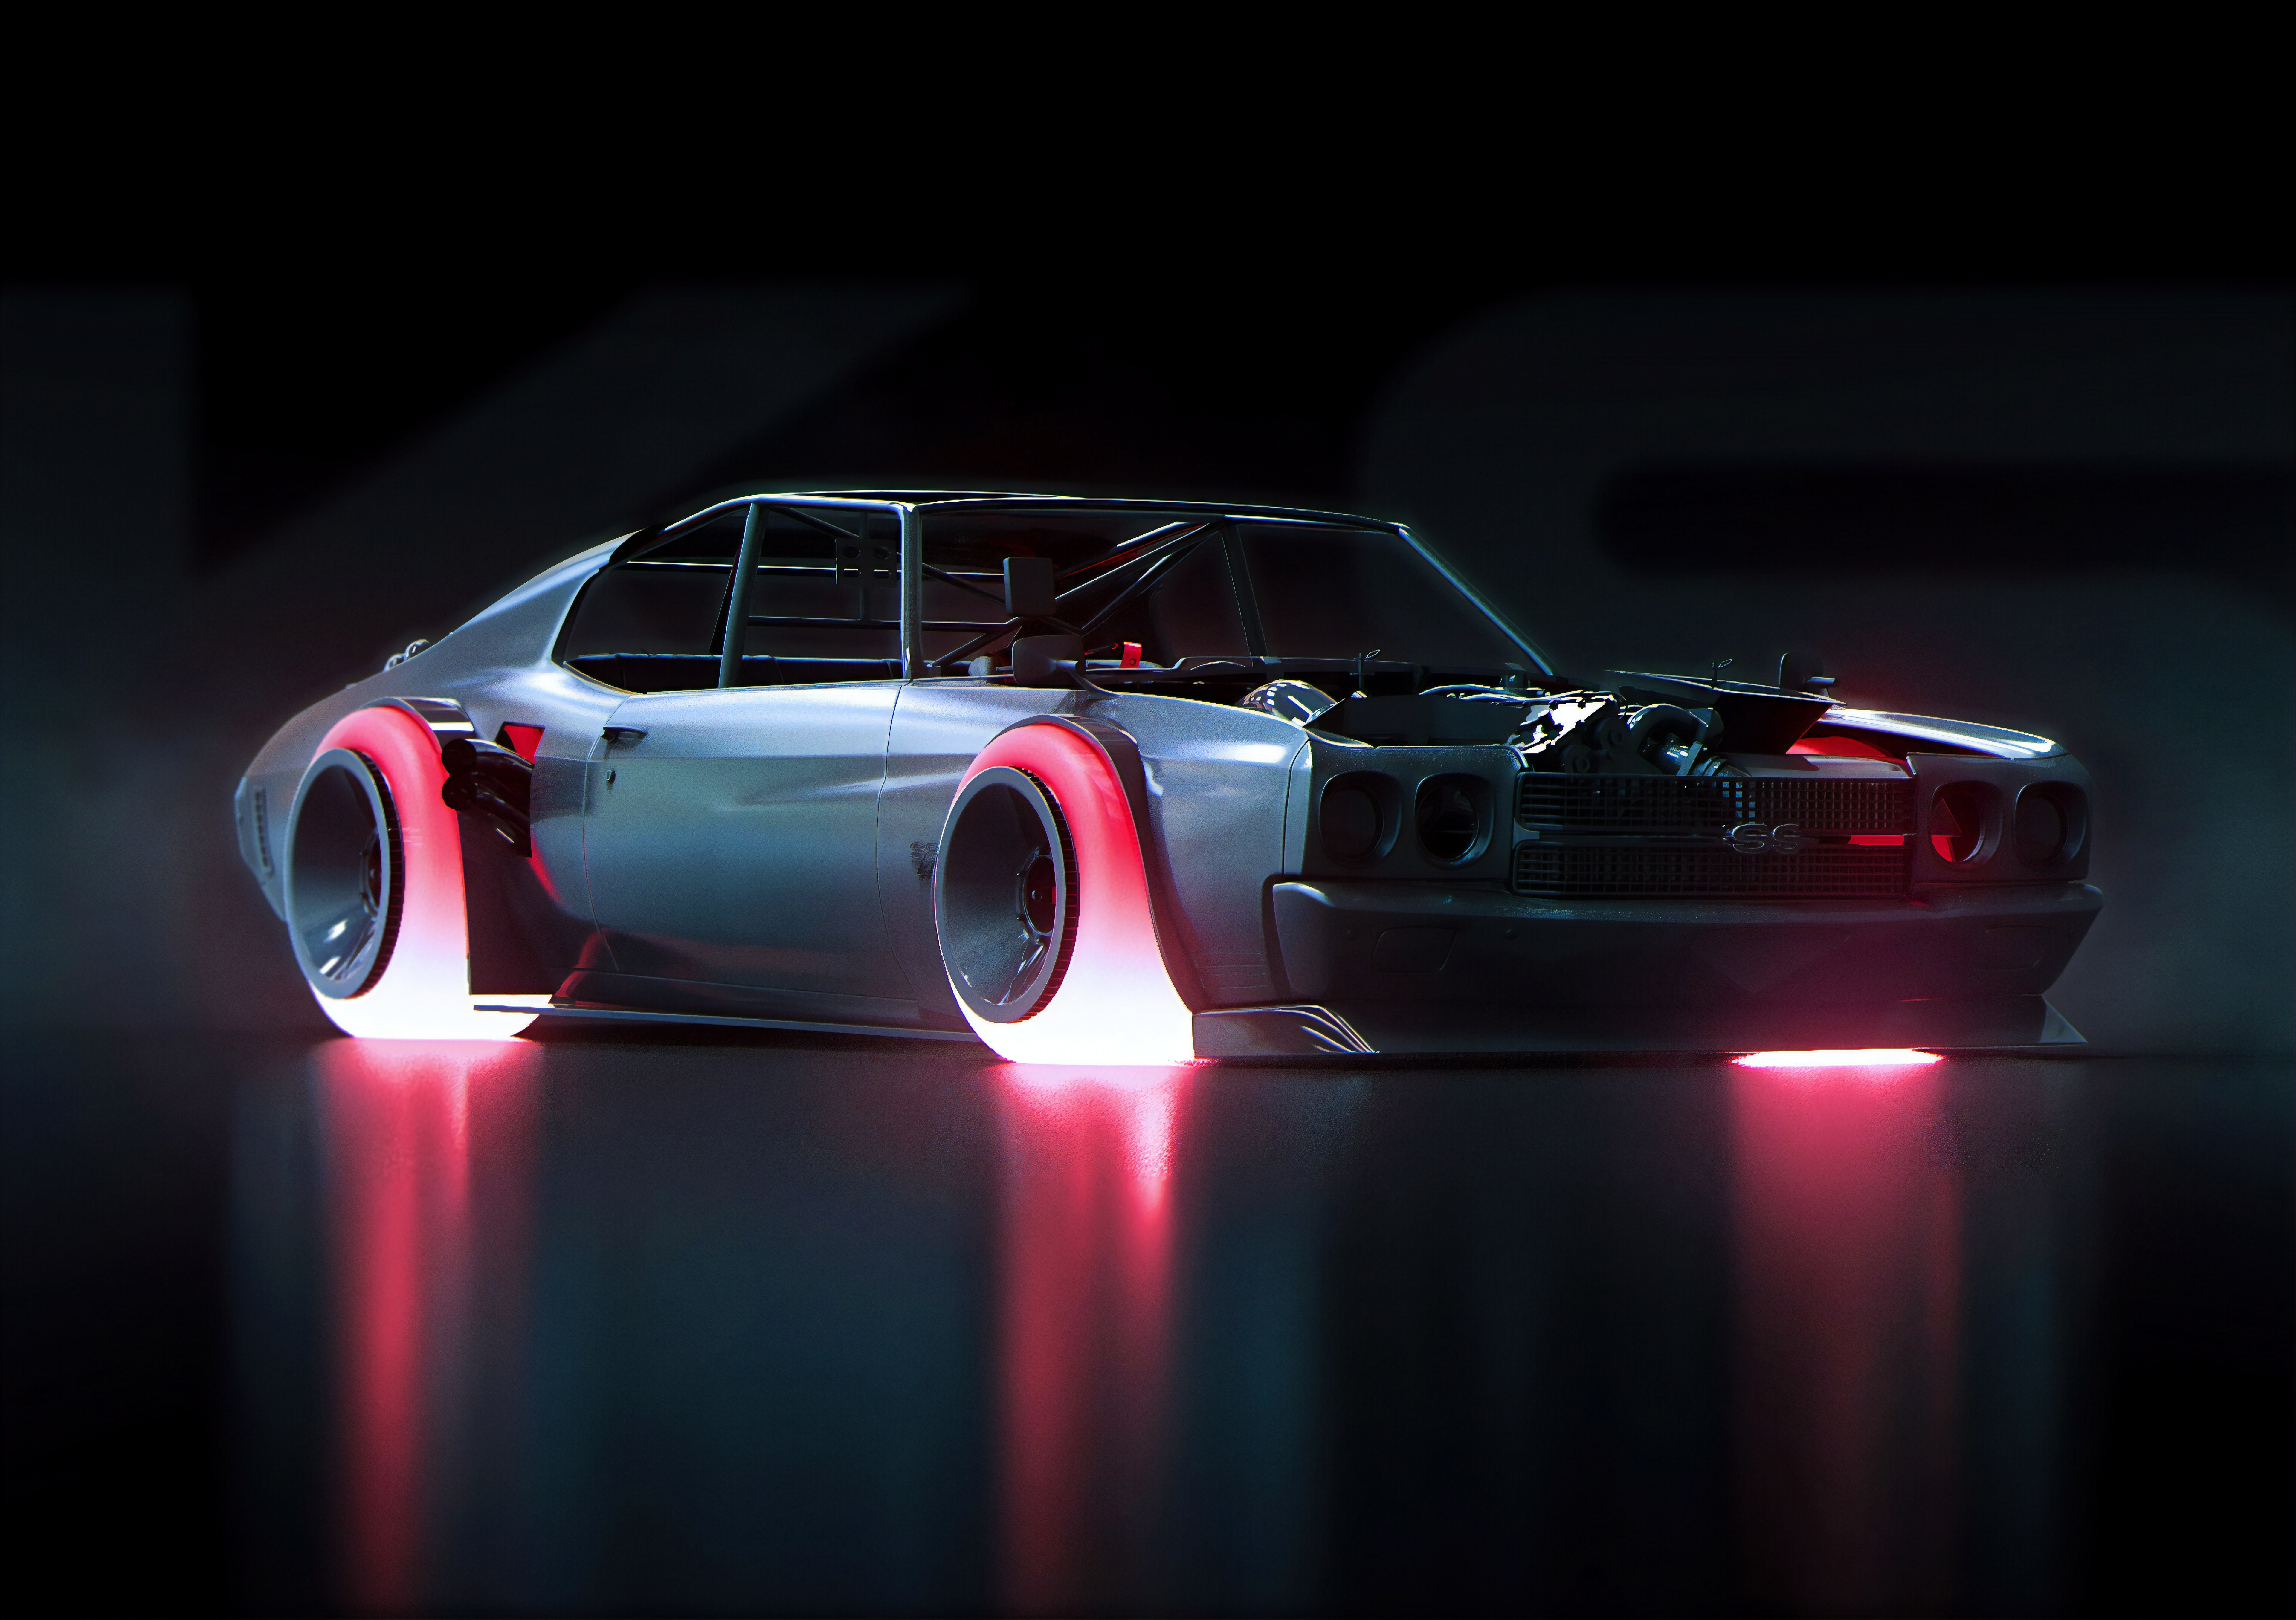
\includegraphics[height=\textwidth,angle=90]{7.jpg}
					\caption*{图12 焊接效果图(反面)}
				\end{minipage}
				\qquad
				\begin{minipage}{0.35\textwidth}
					\centering
					
\includegraphics[height=\textwidth,angle=-90]{8.jpg}
					\caption*{图13 焊接效果图(正面)}
				\end{minipage}
			\end{figure}
			\item 电路功能测试和验证 \par 
			\qquad 在制板和焊接完成之后,需要进行电路功能的测试和验证。首先先通过预留的电源导线接入5V直流电压,然后用手遮住光敏电阻,发现当光敏电阻慢慢被遮住后,发光二级管的亮度慢慢变亮。这是如果再调节电位器时,电路对外界光线的敏感度会发生变化,再用电流表和电压表测电路中各个点的电流和电压,均正常。\par 
			\qquad 电路验证过程见图14 和图15 \par 
			\begin{figure}
				\centering
				\begin{minipage}{0.4\textwidth}
					\centering
					\includegraphics[width=\textwidth]{9.png}
					\caption*{图14 LED亮度随外界变化}
				\end{minipage}
				\qquad
				\begin{minipage}{0.4\textwidth}
					\centering
					\includegraphics[width=\textwidth]{10.png}
					\caption*{图15 手动更改电路敏感度}
				\end{minipage}
			\end{figure}
	\end{enumerate}
	\section*{三、实验结果}
	\begin{enumerate}
		\item 仿真结果 \par 
		\qquad 电路仿真能够正常运行,并且各节点电流和电压均无异常,充放电时间合理,555芯片能够随着光敏电阻或者滑动变阻器的变化,输出相应具有一定占空比的波形。
		\item 实物测试结果 \par 
		\qquad 电路能够顺利导通并工作,电路中个元件均正常工作,没有过压过流烧坏的情况,接入电源后,各点电压和电流正常,并且发光二极管能够随着环境光线的变化调整亮度,并且也能通过调节滑动变阻器手动调节亮度。
	\end{enumerate}
	\section*{四、结果分析}
	仿真和实物的实验结果都表面,前面的计算,原理分析,以及制板和焊接都完成得较好。但是还有一些不足之处。\par 
	在进行实物测试时,发光二极管的亮度不足,说明发光二极管的电压设计存在欠缺,原因时实验前没有查阅和测量发光二极管的合适电压,并进行更加合适的电阻计算。
	同时,电路的焊盘相对较小,在焊接时容易接触不良。由于是单层板的原因,电路中有一些连接需要飞线处理,但是整个电路的飞线没有处理好,略显凌乱。\par 
	在进行电路设计时,也没有预留测试点,导致测量时不太方便。\par 
	\section*{五、心得体会}
	在整个制作的过程中,从设计到仿真,再到焊接和实验,学到了许多东西,也有许多心得体会
	\begin{enumerate}
		\item 懂得了如何设计电路。\par 
		\qquad 设计电路的第一要点,便是弄清需求和目标,然后就是寻找合适的元件了解原理并进行相关计算。在设计过程中,仿真是很重要的一个步骤,因为仿真可以验证电路的一些基本功能,能够减少不必要的硬件损耗。同时,在设计过程中,遇到错误时要学会仔细排查,找出错误。
		\item 学到了许多软件技巧。\par 
		\qquad 在设计过程中,用到了许多软件进行设计,例如AD,嘉立创EDA,proteus,通过这次课程作业,学会了如何利用这些软件进行原理图绘制,PCB绘制,电路仿真。并且也学到了许多技巧,例如利用AD和嘉立创的自动布线功能,可以迅速完成PCB布线;利用DRC检查可以避免一些低级性错误。
		\item 体验并亲手实践了制板工艺。\par 
		\qquad PCB作为一项伟大的发明,是重要的电子部件,是电子元器件的支撑体,通过这次实践,利用实验室资源,我们亲身体会并操作了基本的制板流程,学习到了许多关于制板的知识,为我们以后的进一步工程实践打下基础。
		\item 学会了团队合作 \par 
		\qquad 在本次的实践中,两个人进行团队合作共同完成一个作品。这锻炼了我们的团队合作技巧,两个人的思想如何沟通交流,如何确定项目方案,如何进行分工合作,如何处理合作过程中出现的问题等等。本次课程作业充分锻炼了我们团队意识和团队合作能力。
	\end{enumerate}
\end{document}
